
\chapter{Dislocations in MAX phases}

\label{chap:dislocations_in_max_phases}
\graphicspath{{dislocations_in_max_phases/Figs/}}






In Chapter~\ref{chap:hetero_max_phases} elastic heterogeneity of the unit cell was discussed and the local elastic properties were shown to have a strong dependence on the chemical environment. As discussed in  Chapter~\ref{chap:plastic_deformation} and shown in Chapter~\ref{chap:peierls_model}, the Peierls stress (i.e.\ the lattice resistance at \SI{0}{\kelvin}) is very sensitive to the elastic properties of a crystal. Thus the elastic heterogeneity is expected to have a strong effect on the dislocations in the MAX phases.

The elastic properties of the different layers of the MAX phases are not in the form of full elastic tensors so the approach taken in Chapter~\ref{chap:peierls_model} to use the full strain state cannot be applied. Instead a simplified model, adapted from that presented by \citet{Clegg2006} is used that relies on only simple strains and elastic constants. This model was shown to be in good agreement with experiment across orders of magnitude of the Peierls stress for a wide range of materials and is used here to demonstrate the effects of elastic heterogeneity on the Peierls stress.


\section{Adapted Peierls model}

The lack of a full elastic tensor means that the Peierls model used in this case was adapted from the one published by \cite{Clegg2006}. This works in a similar way to the model described in \ref{chap:peierls_model} except only the first layer of atoms either side of the slip plane are considered and the only displacements allowed are parallel to the Burgers vector, in analogy with the original Peierls model.

The calculation essentially the same; the energy is still a balance between two energy contributions: the elastic energy in the bonds outside the slip plane and the misalignment energy of those bonds across the slip plane. The Peierls stress is then the maximum gradient of the energy changes as the dislocation is displaced. However some aspects are different.


The original model was written to calculate the misalignment energy using the Frenkel approximation, as given in \autoref{eqn:Frenkel_approx}, but the adapted model was extended to use a parametrised $\gamma$-surface to represent the misalignment energies, as represented by the summation
\begin{equation}
\gamma = \sum_{m=1}^{M} C_m \left[ 1 - \cos \left( \frac{2m\pi \phi}{b} \right) \right]\label{eqn:gamma_surface}
\end{equation}
where $\gamma$ is the energy in \si{\joule\per\meter\squared}, $C_m$ are a series of parameters fitted by a least-squares method to a set of energies at different misalignments, $m$ is an integer between 1 and some maximum $M$ which is chosen to be the lowest number that adequately captures the energy profile of the $\gamma$-surface, $b$ is the Burgers vector and $\phi$ is the misalignment in units of \si{\angstrom}, such that $\phi/b$ defines a sort of fractional misalignment. It was generally found that $M=3$ was sufficient to capture the shape of the $\gamma$-surface, but was sometimes extended to six.

The other major difference is that the model in \cite{Clegg2006} optimises the structure of the dislocation only at the equilibrium position, not at every sampled displacement. The adapted model optimises the structure of the dislocation for every position by searching for the dislocation width that yields the lowest dislocation energy.


The elastic moduli and unit cell geometries, both required for the Peierls model, of the regions of the MAX phase structures were calculated in Chapter~\ref{chap:hetero_max_phases} so the only other required input for the model is the misalignment potential, derived from the $\gamma$-surface.

\section{Calculating the \texorpdfstring{$\gamma$}{gamma}-surface}


The density functional theory calculations used the same initial set-up as discussed in \autoref{sec:DFT_method}, based on the equilibrated unit cells with periodic boundary conditions in all directions. To calculate the gamma surfaces, a displacement across a plane must be imposed. The simplest way to do this is to maintain the periodic boundary conditions and introduce two opposing stacking faults, as shown schematically in \autoref{fig:DFT_gamma_surface}. There will be a dependence of the stacking fault energy on the distance between stacking faults, so the simulation must be converged with respect to this distance. In practice the lattice parameter of the MAX phases is long enough that only one or two unit cell repeats were necessary.

\begin{figure}
\centering
\captionsetup{width=0.45\textwidth}
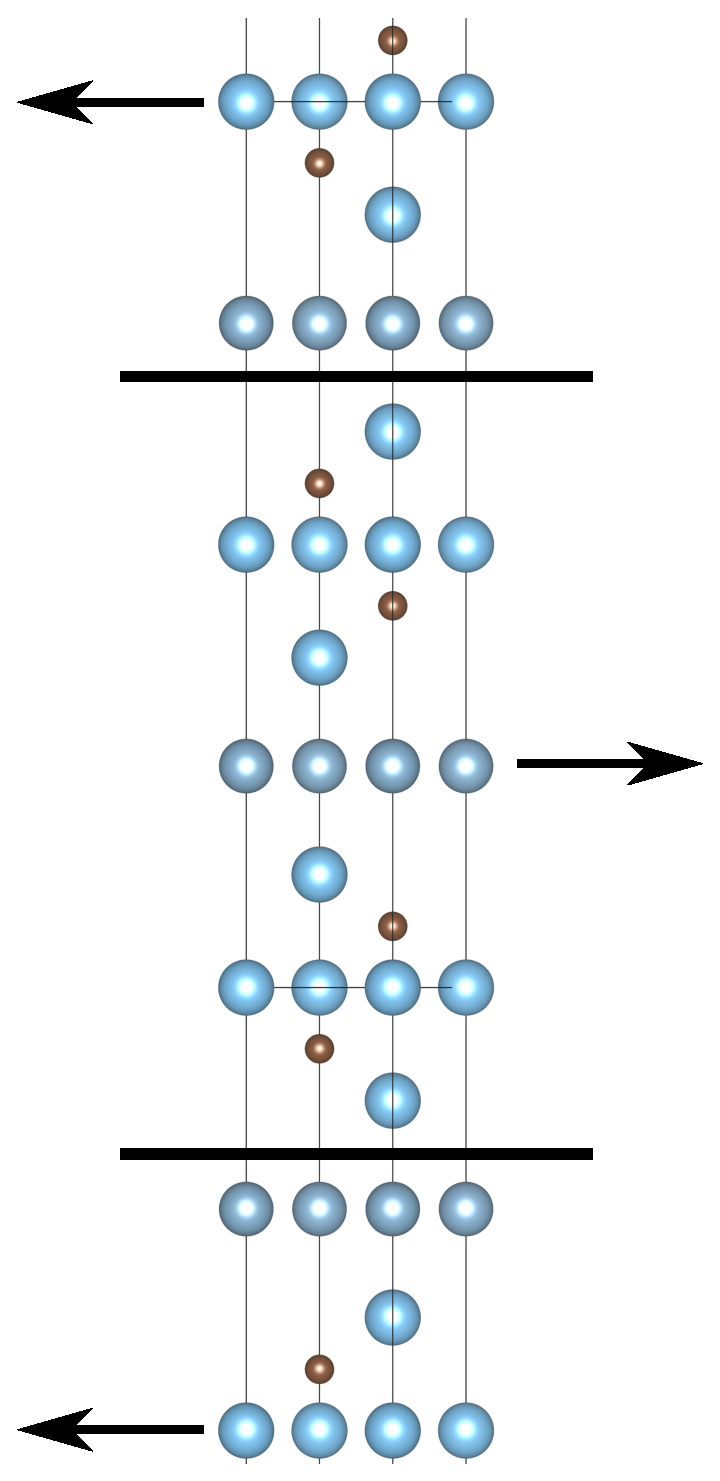
\includegraphics[width=0.3333\textwidth]{displacements_for_gamma_surface}
\caption[Schematic displacements during the simulation of the \texorpdfstring{$\gamma$}{gamma}-surface.]{Schematic showing the displacements applied to a slab of crystal within a periodic cell to create two opposing stacking faults. The energy changes of the system are therefore twice the $\gamma$-surface. Graphic prepared with VESTA \cite{Momma2011}.\label{fig:DFT_gamma_surface}}
\end{figure}

To displace the atoms, SIESTA's Z-matrix was used \cite{SIESTA_manual}. This allows the coordinates of the atoms to be constrained separately in each direction; the displacement parallel to the slip direction, $a/3$<1\,1\,\={2}\,0> was imposed and the atomic positions were relaxed perpendicular to this displacement. This is important as unreasonably close atomic positions would occur without this relaxation. In analogy with the FCC metals it might be expected for there to be a stable stacking fault. The M--A layer can be seen as a single repeat of the HCP structure, with ABA stacking; the faulted stacking, relative to the other M--A layer in the unit cell, is then ACA, see \autoref{fig:MAX_unit_cells}. 

In materials like aluminium dislocations are know to separate into partial dislocation pairs because the stacking fault energy is low enough that dissociating one full dislocation to become two partials reduces the overall energy despite the introduction of a stacking fault \cite{kelly2012ch9}. Atoms are therefore displaced along two successive <2\,1\,1> type directions that sum to <1\,0\,1> overall. Even in the case of full dislocations in close-packed structures this kind of lateral displacement is likely in the core. 

Since the hexagonal structure of the MAX phases would have analogous stacking faults, we can expect a metastable point in the middle of the $\gamma$-surface, corresponding to the stable stacking fault energy, with a substantial lateral displacement of atoms. The Peierls model, either the one developed in Chapter~\ref{chap:peierls_model} or its predecessors \cite{Clegg2006, Howie2017}, cannot account for this so it must be accounted for during the calculation of the $\gamma$-surface.

Initially 40 positions were modelled at regular intervals between one perfect position and the next displacing along the <1\,1\,\={2}\,0>. The energy changes, relative to the equilibrium position, were fitted to the function given in \autoref{eqn:gamma_surface} using the ``\texttt{scipy.curve\_fit}'' package provided by the SciPy project \cite{SciPy2001}.





\section{Results and discussion}

\subsection{The \texorpdfstring{$\gamma$}{gamma} surface}
The results of the DFT calculation of the $\gamma$-surfaces are presented in \autoref{fig:gamma_surfaces} and summarised in \autoref{tab:gamma_surface_params}. \autoref{fig:gamma_surfaces} shows some of the extremes in the calculated $\gamma$-surfaces as well as the $\gamma$-surfaces of some of the more commonly studied MAX phases. 


\begin{table}
%\footnotesize
\centering
\begin{tabular}{|l|c|c|c|c|c|c|}
\hline
   Phase\rule[3ex]{0pt}{0pt} &        C1 &        C2 &        C3 &        C4 &        C5 &        C6 \\
\hline
  \ce{Ti2AlC} \rule[3ex]{0pt}{0pt}  &  0.282992 &  0.156480 & -0.016174             &  \hphantom{-}0.001095 & -0.001666             &  \hphantom{-}0.002269 \\
  \ce{Nb2AlC}                       &  0.448371 &  0.149654 & -0.032832             &  \hphantom{-}0.010283 &  \hphantom{-}0.001951 & -0.001647 \\
 \ce{Ti3SiC2}                       &  0.518409 &  0.165415 & -0.028071             &  \hphantom{-}0.007997 &  \hphantom{-}0.002995 & -0.002455 \\
  \ce{Nb2GaC}                       &  0.308173 &  0.149612 & -0.029413             &  \hphantom{-}0.006746 &  \hphantom{-}0.002960 & -0.002059 \\
  \ce{Nb2InC}                       &  0.224446 &  0.155834 & -0.023865             &  \hphantom{-}0.002967 &  \hphantom{-}0.002511 & -0.001017 \\
   \ce{Nb2SC}                       &  0.556995 &  0.151700 &  \hphantom{-}0.012813 &  \hphantom{-}0.016965 &  \hphantom{-}0.002000 &  \hphantom{-}0.002431 \\
  \ce{Nb2SnC}                       &  0.306205 &  0.112250 &  \hphantom{-}0.013072 &  \hphantom{-}0.003043 & -0.002861             & -0.000279 \\
  \ce{Ti2GaC}                       &  0.203826 &  0.106754 & -0.015401             & -0.000080             &  \hphantom{-}0.001344 & -0.000344 \\
  \ce{Ti2InC}                       &  0.212131 &  0.136290 & -0.019126             &  \hphantom{-}0.001000 &  \hphantom{-}0.001751 &  \hphantom{-}0.000058 \\
   \ce{Ti2SC}                       &  0.480254 &  0.326211 & -0.041373             &  \hphantom{-}0.025800 &  \hphantom{-}0.001488 & -0.000562 \\
  \ce{Ti2SnC}                       &  0.295972 &  0.124439 & -0.017660             &  \hphantom{-}0.002200 &  \hphantom{-}0.000554 & -0.000501 \\
  \ce{Zr2InC}                       &  0.091959 &  0.095488 &  \hphantom{-}0.010618 &  \hphantom{-}0.002890 & -0.001593             & -0.000152 \\
   \ce{Zr2SC}                       &  0.255379 &  0.312817 & -0.021624             &  \hphantom{-}0.016800 &  \hphantom{-}0.001213 &  \hphantom{-}0.000362 \\
  \ce{Zr2SnC}                       &  0.257600 &  0.135233 & -0.019346             &  \hphantom{-}0.002700 &  \hphantom{-}0.002464 & -0.001410 \\
 \ce{Ti3AlC2}                       &  0.283378 &  0.137157 & -0.009093             &  \hphantom{-}0.002380 & -0.000999             & -0.000026 \\
 \ce{Nb4AlC3}                       &  0.439674 &  0.140072 & -0.031167             &  \hphantom{-}0.012671 &  \hphantom{-}0.000282 & -0.001988 \\
 \ce{Ti4SiC3} \rule[-1ex]{0pt}{0pt} &  0.503656 &  0.159172 & -0.026991             &  \hphantom{-}0.007960 &  \hphantom{-}0.002571 & -0.001520 \\
\hline
\end{tabular}
\captionsetup{width=1.2\textwidth}
\caption[\texorpdfstring{$\gamma$}{gamma}-surface results]{Results of the DFT simulation of the $\gamma$-surface for various MAX phases, presented as parameters for \autoref{eqn:gamma_surface}. \label{tab:gamma_surface_params}}
\end{table}


All the $\gamma$-surfaces showed a minimum at $\phi / b = 1/2$, the deepest minima were those in \ce{Ti2SC} and \ce{Zr2SC}. Interestingly the phase \ce{Nb2SC} does not show a similar, pronounced local minimum. The MAX phase closest to showing no local minimum in the stacking fault energy at the anti-phase position is \ce{Nb2SnC}, though even that phase has a small minimum.  This minimum can be explained in terms of the crystal structure. Because the M--A is locally hexagonally close-packed there must exist a stacking fault that alters the sequence from ABA to ACA. This is likely to be a stable stacking fault, i.e. a local minimum in energy, by analogy with hexagonal metallic elements. The existence of the minimum in all the phases shows the importance of the relaxation of the atomic positions perpendicular to the misalignment displacement: a stacking fault could not be formed unless atoms were allowed to move normal to the imposed displacement.


\begin{figure}[!htb]
\centering
\begin{subfigure}{5cm}
\centering
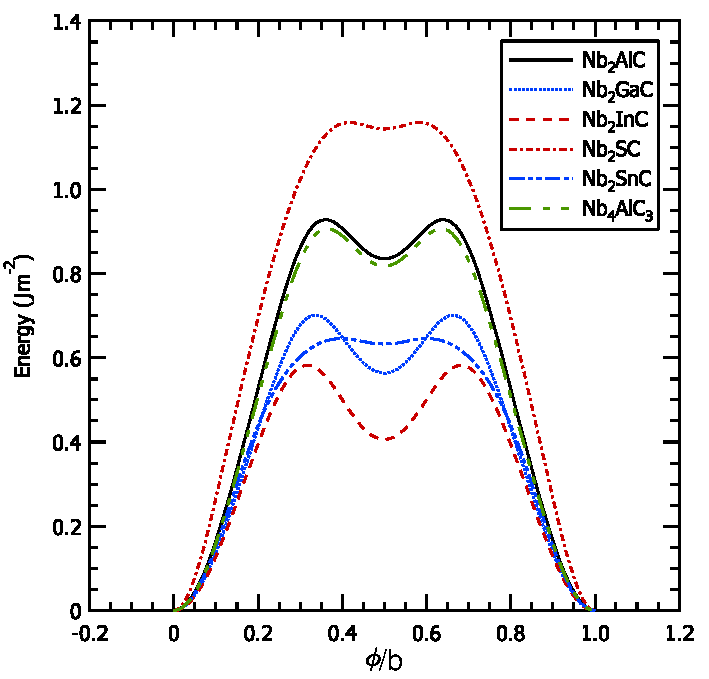
\includegraphics[width=\textwidth]{Nb_gamma_surfaces}
\caption{The $\gamma$-surfaces for the niobium bearing MAX phases.\label{fig:Nb_gamma_surfaces}}
\end{subfigure}
~
\begin{subfigure}{5cm}
\centering
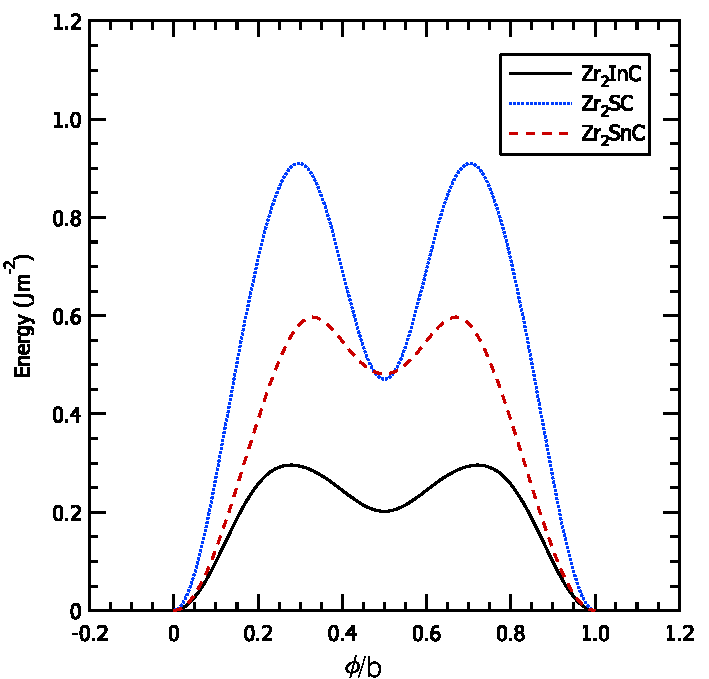
\includegraphics[width=\textwidth]{Zr_gamma_surfaces}
\caption{The $\gamma$-surfaces for the zirconium bearing MAX phases.\label{fig:Zr_gamma_surfaces}}
\end{subfigure}

\begin{subfigure}{5cm}
\centering
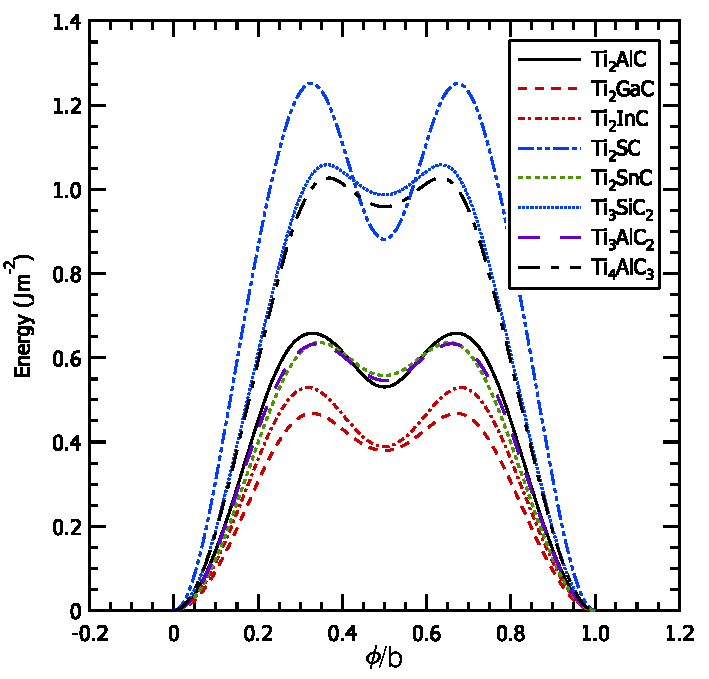
\includegraphics[width=\textwidth]{Ti_gamma_surfaces}
\caption{The $\gamma$-surfaces for the titanium bearing MAX phases.\label{fig:Ti_gamma_surfaces}}
\end{subfigure}

\captionsetup{width=12cm}
\caption[The \texorpdfstring{$\gamma$}{gamma}-surfaces of the MAX phases.]{The $\gamma$-surfaces of the MAX phases, organised by the element occupying the M-site and plotted using the parameters given in \autoref{tab:gamma_surface_params} and the function given in \autoref{eqn:gamma_surface}. \label{fig:gamma_surfaces}}
\end{figure}


The $\gamma$-surfaces show a similar trend to the shear moduli of the M--A layers, as discussed in Chapter~\ref{chap:hetero_max_phases}. The sulphur bearing phases are the tallest and steepest as might be expected from the very low electronegativity difference in those phases, while indium bearing phases, which have the largest electronegativity differences, were the shallowest and other phases taking intermediate positions as expected. More detailed analysis of the $\gamma$-surfaces was undertaken by examining the effect upon the Peierls stress.


\subsection{Lateral motion}



The qualitative nature of the stacking faults was investigated with the VESTA visualisation software and SIESTA's crystal structure export functionality. A series of atomic configurations at increasing misalignments from a value of $\phi/b$ of \numrange{0}{0.5} is shown in \autoref{fig:lateral_motion_stacking_fault}.


\begin{figure}[!ht]
\centering
\includegraphics[width=0.8\textwidth]{gamma}
\captionsetup{width=0.9\textwidth}
\caption[Atomic configurations around stacking faults.]{The atomic positions in \ce{Ti2AlC} projected down the [0\,0\,0\,1] direction as a stacking fault is introduced by displacing a slab of crystal in the unit cell. The displacement is imposed  parallel to [1\,0\,0\,0] and varies from zero to half the Burgers vector. Atoms are allowed to relax normal to the [1\,0\,0\,0]. The atoms initially at the sites marked * and $\dagger$ move laterally as the displacement increases until they are aligned at the position marked $\ddagger$. This is the stable stacking fault and is responsible for the local minimum in the stacking fault energy as seen in \autoref{fig:gamma_surfaces}. Graphics prepaed with VESTA \cite{Momma2011}.\label{fig:lateral_motion_stacking_fault}}
\end{figure}




The two slabs either side of the stacking fault showed clear and substantial lateral displacements. This is shown in \autoref{fig:lateral_motion_stacking_fault} as layers that start initially offset by 1/3[\={1}\,1\,\=2\,0] are aligned when the two slabs are displaced by $b/2$, i.e. half the repeat distance. This lateral motion, and subsequent change of the stacking sequence, represents the stable stacking fault. This is as expected by analogy with hexagonal close-packed structures. The combination of the lateral motion with the displacement parallel to the slip direction, [1\,0\,\={1}\,0], means that the atoms follow a trajectory along the Burgers vectors of two partial dislocations as shown in \autoref{fig:lateral_motion_stacking_fault}. This is exactly as would be expected from the similarity of the M--A layer to the hexagonal close-packed crystal structure. 


\subsection{Peierls stress}

The Peierls stress is shown against the lattice geometry, as defined by $d/b$, in \autoref{fig:peierls_stress_vs_d_upon_b}. There is a huge range in the predicted Peierls stress: $\tau_p / G$ varies from \numrange{4.07d-3}{1.29d-5} for \ce{Ti2SC} and \ce{Zr2InC} respectively. In absolute terms this is a range of $\sim$\SIrange{1}{690}{\mega\pascal} for those same phases. All the calculated Peierls stresses are lower than would be expected from the lattice geometries, i.e. $d/b$, alone.



\begin{figure}
\centering
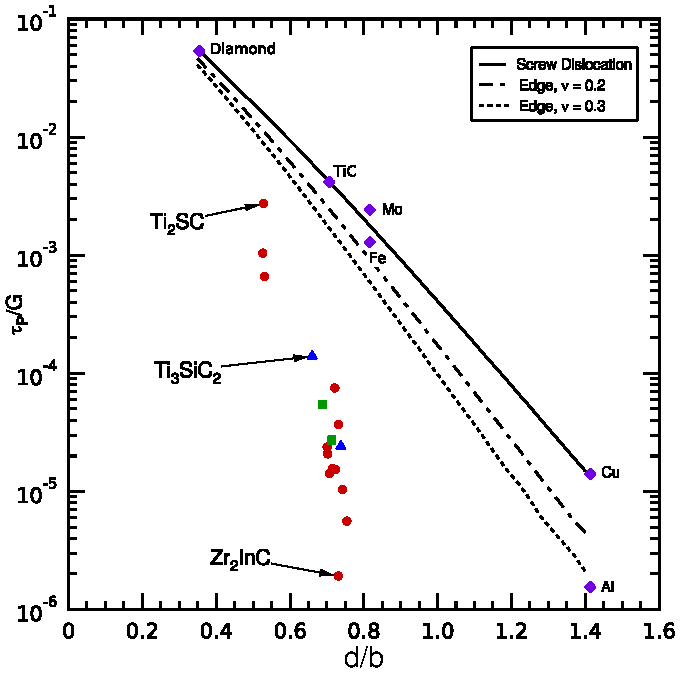
\includegraphics[width=10cm]{tp_vs_d_upon_b}
\captionsetup{width=12cm}
\caption[The calculated Peierls stresses of the MAX phases.]{The calculated Peierls stress, normalised by the shear modulus, against $d/b$ for the MAX phases. This defines the lattice resistance at \SI{0}{\kelvin}. The circles, triangles and squares represent the 211, 312 and 413 phases respectively, the diamonds are some reference phases with simpler crystal structures, with values obtained from \cite{Clegg2006}. The lines show the prediction for an isotropic elastic medium for a screw dislocation and an edge dislocation for two different values of the Poisson ratio. \label{fig:peierls_stress_vs_d_upon_b}}
\end{figure}


Some variation is expected as the lattice geometry changes across the MAX phases, as discussed in Chapter~\ref{chap:hetero_max_phases} increasing the electronegativity difference between the layers of the crystal structure leads to a shortening of the M--A bond length, which in turn reduces the value of $d/b$. The range in $d/b$ observed in the MAX phases, about \numrange{0.5}{0.75}, would account for a reduction in $\tau_p / G $ by around a factor of \num{10} in an isotropic material, however the MAX phases exhibit a drop of around \num{300} times. Hence there is also a greater variation in the predicted Peierls stress than can be accounted for by the variation in the crystal structure alone. 


The variation of the Peierls stress with the electronegativity difference across the structure is shown in \autoref{fig:tp_vs_dX}. Increasing electronegativity difference between the M--X and the M--A layers clearly correlates well with a large decrease in the Peierls stress. As was discussed earlier, in Chapter~\ref{chap:plastic_deformation}, the structure of a dislocation is key to its properties. In particular the Peierls stress is exponentially dependent on the width of the dislocation core, with wide dislocations gliding easily and narrow dislocations exhibiting a large resistance. The variation of the dislocation width is shown against the electronegativity difference in \autoref{fig:w0_vs_dX} and against the ratio of the shear moduli between the regions of the unit cell in \autoref{fig:w0_vs_Gma_upon_Gmx}.




\begin{figure}
\centering
\begin{subfigure}{7.5cm}
\centering
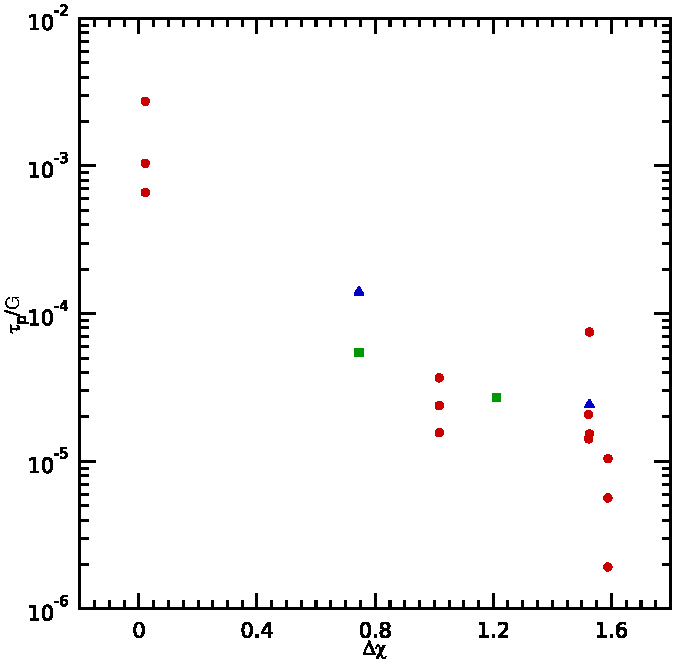
\includegraphics[width=6.6cm]{tp_vs_dX}
\caption{The variation of normalised Peierls stress with the electronegativity difference within the crystal structure.\label{fig:tp_vs_dX}}
\end{subfigure}
\par\medskip
\begin{subfigure}{7.5cm}
\centering
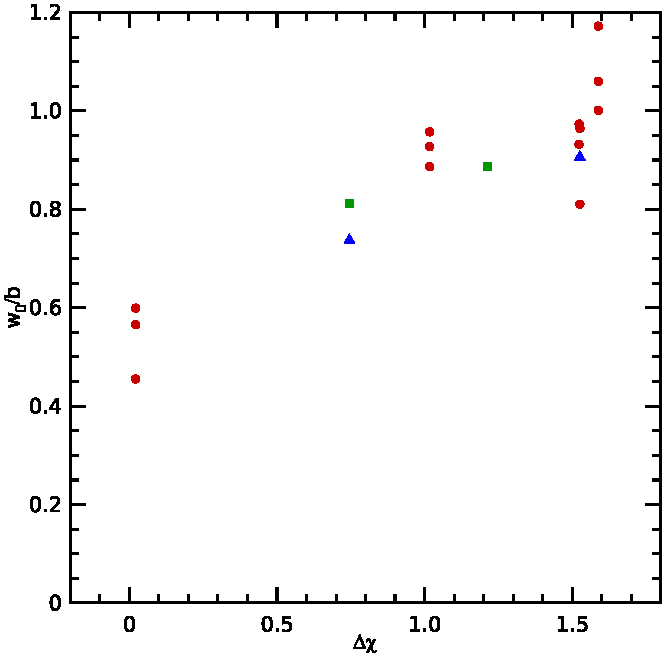
\includegraphics[width=6.6cm]{w0_vs_dX}
\captionsetup{width=\textwidth}
\caption{The variation of the dislocation width, at the equilibrium position, with the difference in electronegativity between the layers of the MAX phase structure.\label{fig:w0_vs_dX}}
\end{subfigure}
\par\medskip
\begin{subfigure}{8cm}
\centering
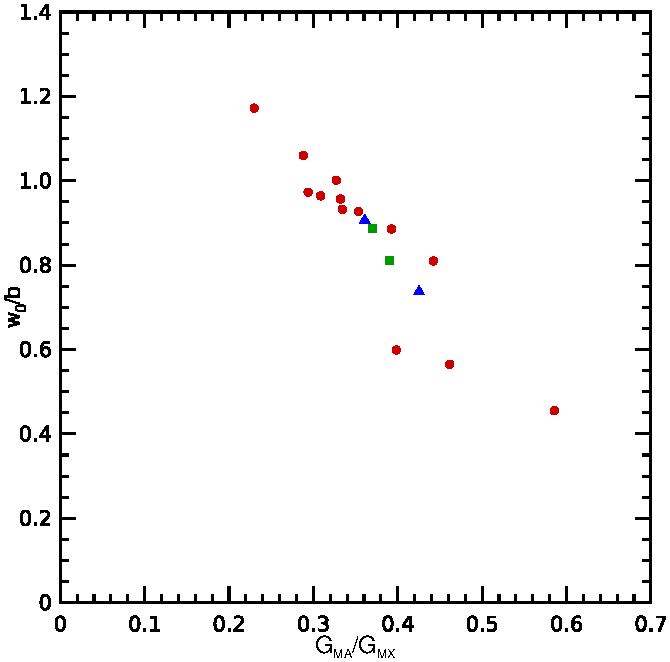
\includegraphics[width=6.6cm]{w0_vs_Gma_upon_Gmx}
\caption{The variation of the dislocation width, at the equilibrium position, with the ratio of the shear moduli of the M--A and M--X regions of the unit cell. \label{fig:w0_vs_Gma_upon_Gmx}}
\end{subfigure}

\caption[The link between the structure of dislocations and local heterogeneity.]{The link between the chemical heterogeneity, as expressed as an electronegativity difference between regions of the unit cell, and the Peierls stress. This dislocation geometry is dependent on the ratio of the moduli of the M--A and M--X layers, which is controlled by the electronegativity difference as discussed in Chapter~\ref{chap:hetero_max_phases}. \label{fig:structure_of_dislocations}}
\end{figure}


\autoref{fig:structure_of_dislocations} shows that the structure of the dislocation is altered considerably across the range of MAX phases investigated which is expected to have a large impact on the Peierls stress as predicted by Peierls and seen in \autoref{fig:peierls_stress_vs_d_upon_b}. As discussed in \autoref{sec:dislocations}, the size of the dislocation is controlled by the competition between two energetic factors; firstly the strain energy in the crystal away from the slip plane favours a wide dislocation and secondly the misalignment energy in the slip plane favours a narrow dislocation. In the MAX phases the local heterogeneity allows the introduction of a lower misalignment energy and a higher strain energy than would be expected thus stabilising a wide dislocation core.

The strain energy term is raised because the electronegativity difference draws electrons into the M--X layer, stiffening it. Conversely the misalignment energy term, which is characterised crudely by the lower shear modulus or more accurately by the $\gamma$-surface, is lowered by the loss of electrons from the M--A layer which occurs under the influence of the electronegativity difference. Thus increasing the electronegativity difference increases the strain energy term and reduces the misalignment energy term, stabilising a wider dislocation and lowering the Peierls stress.

It is this local juxtaposition of the two heterogeneous regions so close together that creates this heterogeneity softening effect. If the heterogeneity were over a larger length scale than adjacent planes of atoms, the dislocations would be affected much less. The stiff region, which has a high in-plane strain energy in the MAX phases, would also have a high misalignment energy. Similarly the compliant region would have a low strain energy in addition to its low misalignment energy. This would lead to narrower dislocations in either region.





\section{Conclusions}

The generalised stacking fault energy, or $\gamma$-surface, of the MAX phases was investigated with density functional theory both quantitatively and qualitatively. As expected the heterogeneity of the unit cell had a strong influence on the $\gamma$-surface; very heterogeneous phases with a large electronegativity differences had low and shallow $\gamma$-surfaces and more homogenous MAX phases with lower electronegativity differences had higher and steeper $\gamma$-surfaces.

The importance of careful modelling of the $\gamma$-surface was demonstrated. Relaxation of the atomic positions laterally, i.e. perpendicular to the misalignment, created a metastable point in the $\gamma$-surface, associated with following the trajectory of two partial dislocations rather than na\"{i}vely following the Burgers vector. All the phases exhibited this local minimum at the halfway position, corresponding to a stable stacking fault.

The $\gamma$-surfaces were used, along with the elastic results presented in Chapter~\ref{chap:hetero_max_phases}, to calculate the Peierls stress with an adapted version of the Peierls model. The MAX phases were all softer than expected for phases with their lattice geometry and elastic moduli and showed a greater decrease in the Peierls stress with increasing $d/b$ than expected.

The structure of the dislocations was examined and it was found that the increasing electronegativity difference, which drives the variation in the $d/b$ ratio, the heterogeneity of the local elastic moduli and the nature of the $\gamma$-surfaces, is associated with the changes in the dislocation width. Increasing the local heterogeneity results in strengthening of the bonding in the electronegative M--X region and a weakening in the electropositive M--A region, which in turn raises the strain energy term driving wider dislocations and weakens the misalignment energy term driving narrower dislocations. This coupled effect stabilises wider dislocations which glide more easily.


That the low flow stresses in the MAX phases can be explained by the local heterogeneity in the unit cell suggests that controlled chemical heterogeneity in crystal is a route to tailoring the Peierls stress. Since the toughness in many non-metallic materials is limited by the force required to move dislocations, this is also a potential route to increasing the toughness of non-metallic materials.






























